\documentclass[a4paper,12pt]{article}
\usepackage[utf8]{inputenc}
\usepackage[english]{babel}
\usepackage{graphicx}
\usepackage{ragged2e}
\usepackage{geometry}
\renewcommand{\baselinestretch}{1.2}
\usepackage{comment}
\usepackage{amssymb}
\usepackage{hyperref}
\usepackage{url}
\usepackage{listings}
%\usepackage{color}
\usepackage{xcolor}

\begin{comment}
	\usepackage{tikz}
	\usetikzlibrary{shapes.geometric, arrows}
	
	\tikzstyle{startstop} = [rectangle, rounded corners, minimum width=3cm, minimum height=1cm,text centered, draw=black,]
	
	\tikzstyle{io} = [trapezium, trapezium left angle=70, trapezium right angle=110, minimum width=3cm, minimum height=1cm, text centered, draw=black, ]
	
	\tikzstyle{process} = [rectangle, minimum width=3cm, minimum height=1cm, text centered, draw=black, ]
	
	\tikzstyle{decision} = [diamond, minimum width=3cm, minimum height=1cm, text centered, draw=black,]
	
	\tikzstyle{arrow} = [thick,->,>=stealth]
\end{comment}


\definecolor{mygreen}{HTML}{087012}
\definecolor{mygray}{HTML}{7e7f81}
\definecolor{mymauve}{HTML}{cb5be2}

\lstset{ 
	language=Python,
	backgroundcolor=\color{white},  
	basicstyle=\footnotesize,        % size of fonts
	breaklines=true,                 % automatic line breaking
	captionpos=b,                   
	commentstyle=\color{mygreen},    % comment style
	keywordstyle=\color{blue},       % keyword style
	stringstyle=\color{mymauve},     % string literal style
}

\begin{document}
	\begin{center}
		\textbf{Assignment-8 \\
			\bigskip
			ELP - 718 Telecom Software Laboratory \\
			\smallskip
			Pardhi Chandan Waman \\
			2018JTM2248 \\
			2018-2020} \\
		\vspace{10mm}
		A report presented for the assignment on \\
		Python and Github \\
		\vspace{30mm}
		
\includegraphics[scale=0.5]{logo} \\
		\vspace{10mm}
		Bharti School Of \\
		Telecommunication Technology and Management \\
		IIT Delhi \\
		India \\
		September 27, 2018
	\end{center}
	\newpage
	\tableofcontents
	\newpage
	\listoffigures
	\newpage
	
	
	\section{Problem Statement 1}
	\subsection{Problem Statement}
	IIT Delhi, has just got the strongest computer. The professors in charge wants to check the computational capacity of the computer. So, they decided to create the problem which is to be given as an assignment to students. Can you help the professor to check the computation capability of the computer?\\
	
	A valid cross is defined here as the two regions (horizontal and vertical) of equal lengths crossing over each other. These lengths must be odd, and the middle cell of its horizontal region must cross the middle cell of its vertical region.\\
	
	

	\subsection{Program Structure}
	
	
	\begin{figure}[h]
		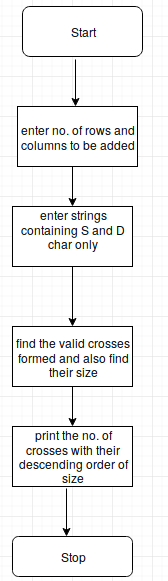
\includegraphics[scale=0.45]{flow1.png}
		\caption{flowchart for ps1}
		\label{fig:flow}
	\end{figure}

	
	\subsection{Algorithm and Implementation}
	\begin{itemize}
		\item create ps1.py to write a code for given problem statement.
		\item take m n i.e. no of rows and col from user
		\item take array of 'S' and 'D' from user.
		\item find the pattern using a code.
		\item output the largest two matching pattern diamentions
		\item stop.
   \end{itemize}
	\subsection{Input and Output format}
	\begin{itemize}
		\item \textbf{Input Format}\\
		The first line contains two space-separated integers,  n and m. 
		Each of the next  lines n contains a string of  m characters where each character is either S (Smart) or D (Dull). These strings represent the rows of the grid. If the jth character in the ith  line is S, then  (i,j) is a  cell smart. Otherwise it's a  dull cell \\
		\textbf{Constraints} \\
	$	2 \leqslant n \leqslant 105 $\\
	$	2 \leqslant m \leqslant 105$ \\
		
		\item \textbf{Output Format}\\
		Find two valid crosses that can be drawn on smart cell of the grid, and return the dimension of both the crosses in the reverse sorted order(i.e. First Dimension should be the larger one and other should be smaller one).
		
	\end{itemize}
	\subsection{Test Cases}
	\begin{enumerate}
		\item 
		5 6 \\
		SSSSSS \\
		SDDDSD \\
		SSSSSS \\
		SSDDSD \\
		SSSSSS \\
		
		\item 
		6 6 \\
		DSDDSD\\
		SSSSSS\\
		DSDDSD\\
		SSSSSS\\
		DSDDSD\\
		DSDDSD\\
		
	\end{enumerate}

	\subsection{Difficulties/Issues Faced}
	In building a logic for the problem statement. Actual implementation in code was difficult to achieve.
	
	\begin{comment}
	\begin{itemize}
		\item 
		\item 
	\end{itemize}
	\end{comment}
	\newpage
	\subsection{Screen-shots}
	
	
		\begin{figure}[h]
		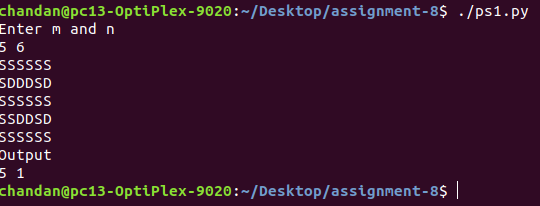
\includegraphics[scale=0.7]{ps1.png}
		\caption{Output for ps1}
		\label{fig:ps1_1}
		\end{figure}
	
	\begin{comment}
		\begin{figure}[h]
		\includegraphics[scale=0.7]{ps1_2.png}
		\caption{ps1- Decision 3}
		\label{fig:ps1_2}
		\end{figure}
		
		\begin{figure}[h]
		\includegraphics[scale=0.6]{ps1_3.png}
		\caption{ps1- Decision 4}
		\label{fig:ps1_3}
		\end{figure}
	\end{comment}
	
	\newpage
	
	\section{Problem Statement 2}

	
	\subsection{Problem Statement}
		After, getting mix results of valid crosses, professors decided to test the computation abilities on one more problem. This time professors wanted to test the decryption capabilities of the computer.
	Encryption of  a message requires three keys, k1, k2, and k3. The 26 letters of English and underscore are divided in three groups,  [a-i] form one group, [j-r] a second group, and everything else ([s-z] and underscore) the third group. Within each group the letters are rotated left by ki positions in the message. Each group is rotated independently of the other two. Decrypting the message means doing a right rotation by ki positions within each group.
	
	\subsection{Assumptions}
	Input string and keys to decrypt a string is available with the user decrypting a string.
	\newpage
	\subsection{Program Structure}
	
	
	\begin{figure}[h]
	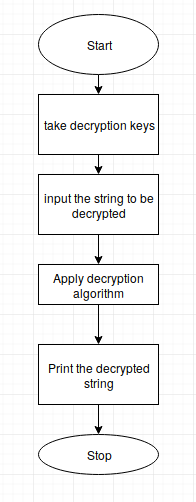
\includegraphics[scale=0.8]{flow2.png}
	\caption{flowchart for ps1}
	\label{fig:flow}
	\end{figure}
	
	\newpage
	\subsection{Algorithm and Implementation}
	\begin{itemize}
		\item Created ps2.py to write a code for decryption algorithm 
		\item key and encrypted string is taken from user.
		\item Decryption algorithm is applied as given in the problem statement.
		\item input Encrypted string along with a key gives Original Decrypted string.
	\end{itemize}
	\subsection{Input and Output format}
	\begin{itemize}
		\item \textbf{Input Format}\\
		Input is key and Encrypted string.
		\item \textbf{Output Format}\\
		Output is Decrypted String
	\end{itemize}
	\subsection{Test Cases}
	\begin{enumerate}
		\item Input
		1 1 1\\
		bktcluajs\\
		\item Output \\
		ajsbktclu
		
	\end{enumerate}
	
	\subsection{Difficulties/Issues Faced}
	Proper ouput is not obtained for some other random strings.
	
	\newpage
	\subsection{Screen-shots}
	
	
	\begin{figure}[h]
	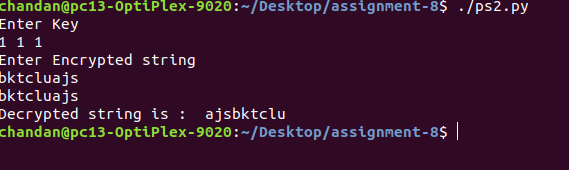
\includegraphics[scale=0.8]{ps2.png}
	\caption{ps2 - Output on Terminal}
	\label{fig:ps2}
	\end{figure}

	\begin{comment}
	\begin{figure}[h]
	\includegraphics[scale=0.7]{ps1_2.png}
	\caption{ps1- Decision 3}
	\label{fig:ps1_2}
	\end{figure}
	
	\begin{figure}[h]
	\includegraphics[scale=0.6]{ps1_3.png}
	\caption{ps1- Decision 4}
	\label{fig:ps1_3}
	\end{figure}
	\end{comment}
	
	
	
	\newpage
	\section{Appendix}
	\subsection{Appendix-A: code for ps1}
	\lstinputlisting{ps1.py}
	\newpage
	\subsection{Appendix-B:code for ps2}
	\lstinputlisting{ps2.py}
	\newpage
	

	\nocite{*}
	\bibliographystyle{amsplain}
	\bibliography{bibreport}
\end{document}